\chapter{Resultados}  \label{cap:resultados}
Este capítulo apresentará os resultados obtidos após a fase de implementação. Inclui a apresentação das funcionalidades do sistema por \textit{print screens} e a descrição dos testes realizados monitorando pedaladas reais.

\section{Apresentação das Funcionalidades do Sistema}
A Figura \ref{fig:printLogin} é um \textit{print screen} do formulário de \textit{login} e a Figura \ref{fig:printHome}, da tela inicial da aplicação, para qual o usuário é redirecionado após o \textit{login} ser realizado com sucesso.

\begin{figure}[h]
\begin{minipage}{.5\textwidth}
    \centering
    \captionof{figure}{GUI de \textit{login}.}
    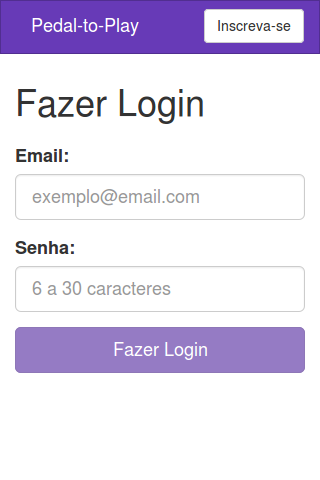
\includegraphics[width=.47\linewidth]{figuras/p2pAuth.png}
    \label{fig:printLogin}
\end{minipage}%
\begin{minipage}{.5\textwidth}
    \centering
    \captionof{figure}{GUI inicial do Pedal-to-Play.}
    \centerline{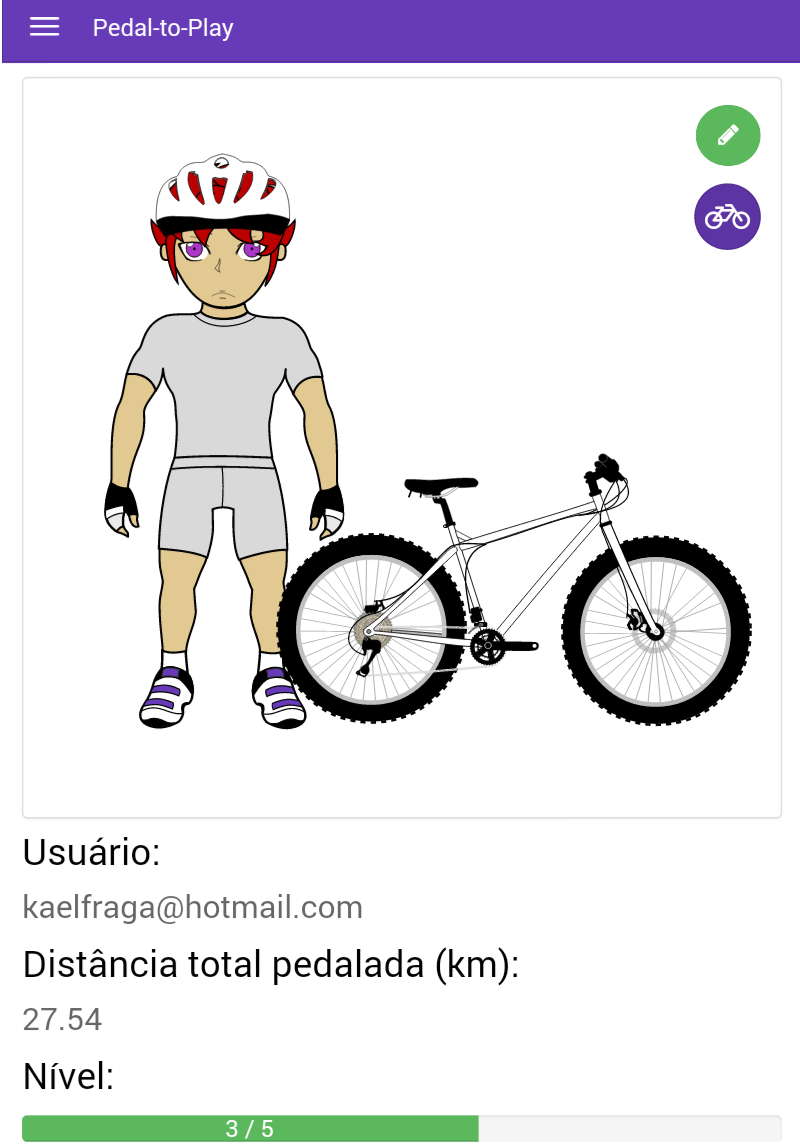
\includegraphics[width=.5\linewidth]{figuras/p2pHome.png}}
    \label{fig:printHome}
\end{minipage}
\par%
\bigskip
\centerline{Fonte: \textit{Print screens} do Pedal-to-Play.}
\end{figure}

Além dos itens especificados na prototipação, a GUI inicial do sistema apresenta os itens "Distância total pedalada" e o botão com ícone de bicicleta. O primeiro informa a soma dos quilômetros percorridos pelo usuário em todas as atividades já monitoradas e o segundo redireciona para a GUI de monitoramento (ou para a GUI de histórico de pedaladas, se o usuário está acessando o sistema via \textit{web page}). Outro detalhe é a informação contida na barra de progresso, correspondente ao nível atual do usuário em relação à quantidade de níveis existentes. 
\par
As Figuras \ref{fig:avatarMobile} e \ref{fig:avatarWeb} correspondem à funcionalidade de customização do avatar virtual respectivamente, para dispositivos com pouca largura de tela (tais como os \textit{smartphones}) e para dispositivos com telas largas (\textit{tablets} e \textit{desktops}).   

\begin{figure}
\begin{minipage}{.4\textwidth}
    \centering
    \captionof{figure}{GUI de customização\\para telas pequenas.}
    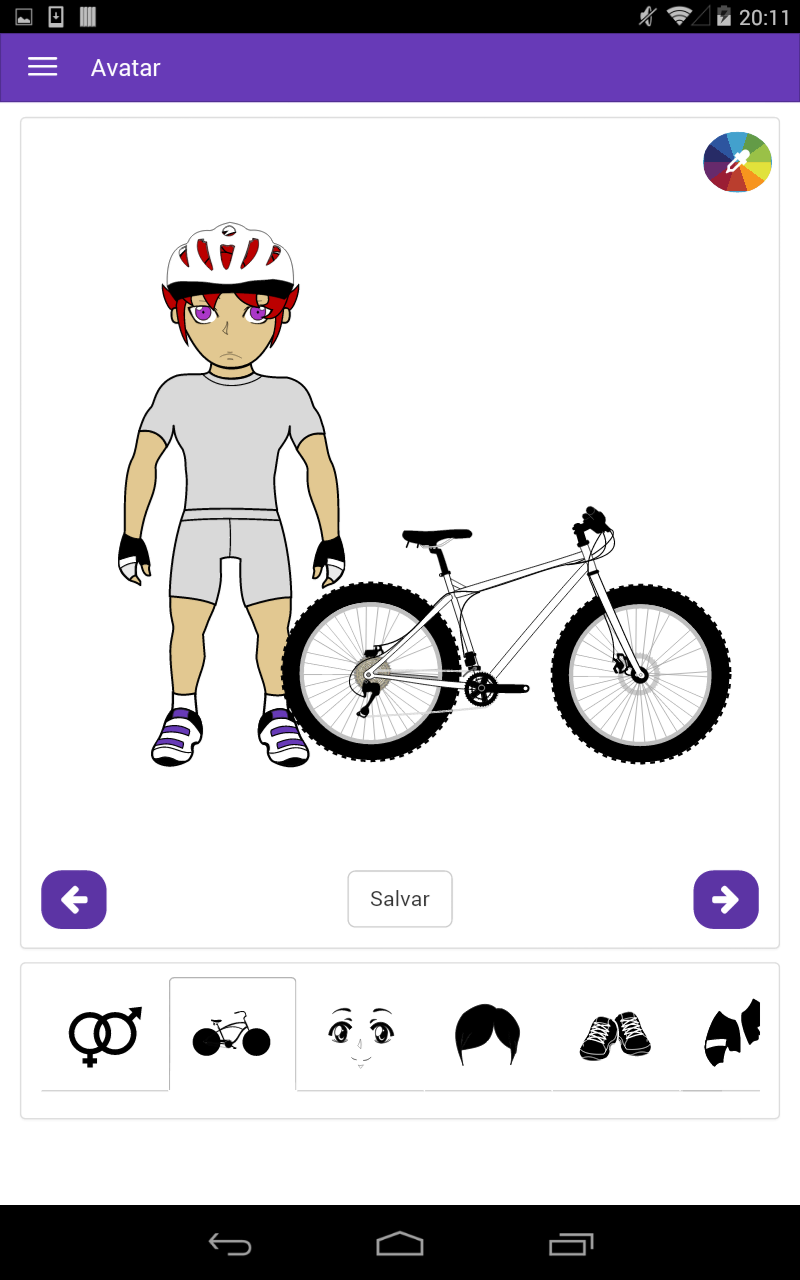
\includegraphics[width=.6\linewidth]{figuras/p2pAvatar.png}
    \label{fig:avatarMobile}
\end{minipage}%
\begin{minipage}{.6\textwidth}
    \centering
    \captionof{figure}{GUI de customização\\para telas grandes.}
    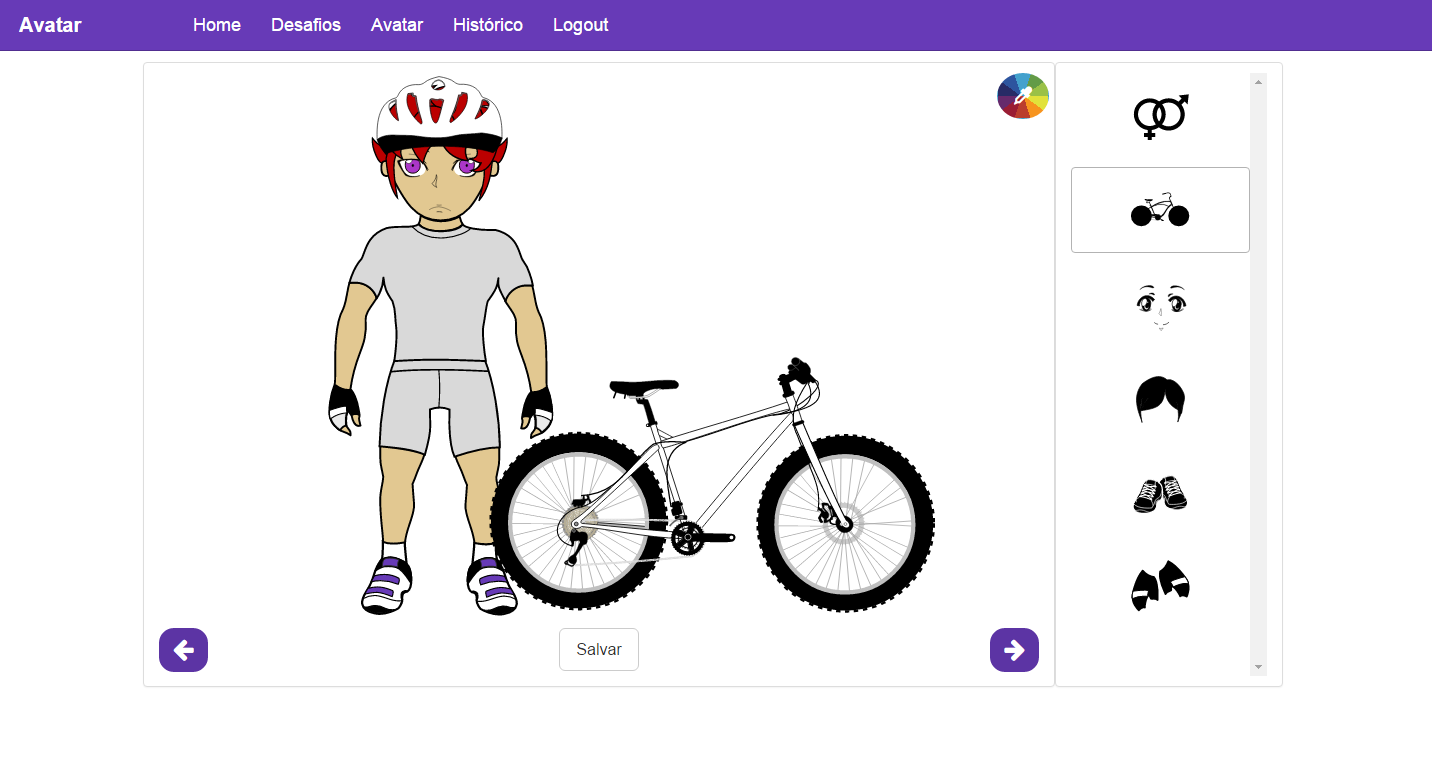
\includegraphics[width=1.1\linewidth]{figuras/p2pWebAvatar.png}
    \label{fig:avatarWeb}
\end{minipage}
\par%
\bigskip
\centerline{Fonte: \textit{Print screens} do Pedal-to-Play.}
\end{figure}

Diferente dos protótipos, a mudança de peças do avatar é realizada selecionando uma categoria de peça entre as disponíveis e usando os botões direcionais para navegar entre as opções de cada categoria.
\par
A Figura \ref{fig:trackingMobile} apresenta a funcionalidade de monitoramento de pedalada em execução, mostrando a velocidade atual do usuário, a distância total percorrida e o tempo total da atividade corrente até o momento do \textit{print screen}.

\begin{figure}[h]
\begin{minipage}{1.0\textwidth}
    \captionof{figure}{Monitoramento de pedalada em execução.}
    \centerline{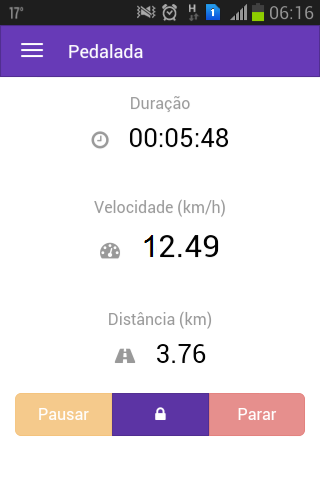
\includegraphics[width=10em]{figuras/p2pTracking.png}}
    \label{fig:trackingMobile}
\end{minipage}
\centerline{Fonte: \textit{Print screen} do Pedal-to-Play.}
\end{figure}

As Figuras \ref{fig:recordsMobile} e \ref{fig:recordsWeb}, respectivamente, apresentam a GUI de visualização do histórico de pedaladas para dispositivos com pouca largura de tela e a GUI para dispositivos com telas largas. 
\par
Ao selecionar uma das atividades contidas na lista "Pedaladas", o mapa é recarregado mostrando o trajeto salvo após o monitoramento da atividade em questão. Cada pedalada na lista é identificada pela sua descrição e a data em que foi salva no sistema. Estas mesmas informações aparecem no mapa como o \textit{label} do marcador localizado sobre o ponto inicial do trajeto da pedalada.
\par
A Figura \ref{fig:questsMobile} apresenta a GUI com os desafios propostos ao usuário. Os desafios possuem \textit{status} (canto superior direito de cada repartição) que indicam se ele já foi completado, se está em andamento ou se ainda não está disponível (caso o nível do usuário seja menor que o nível exigido pelo desafio). Cada repartição contém um desafio, sua descrição, seus requisitos para serem cumpridos e uma pré-visualização das recompensas. O botão inferior à direita redireciona para a GUI de monitoramento, ou histórico de pedaladas, caso o usuário esteja acessado o sistema via \textit{web page}. 

\begin{figure}[h]
\begin{minipage}{.3\textwidth}
    \centering
    \captionof{figure}{Histórico de pedaladas em telas pequenas.}
    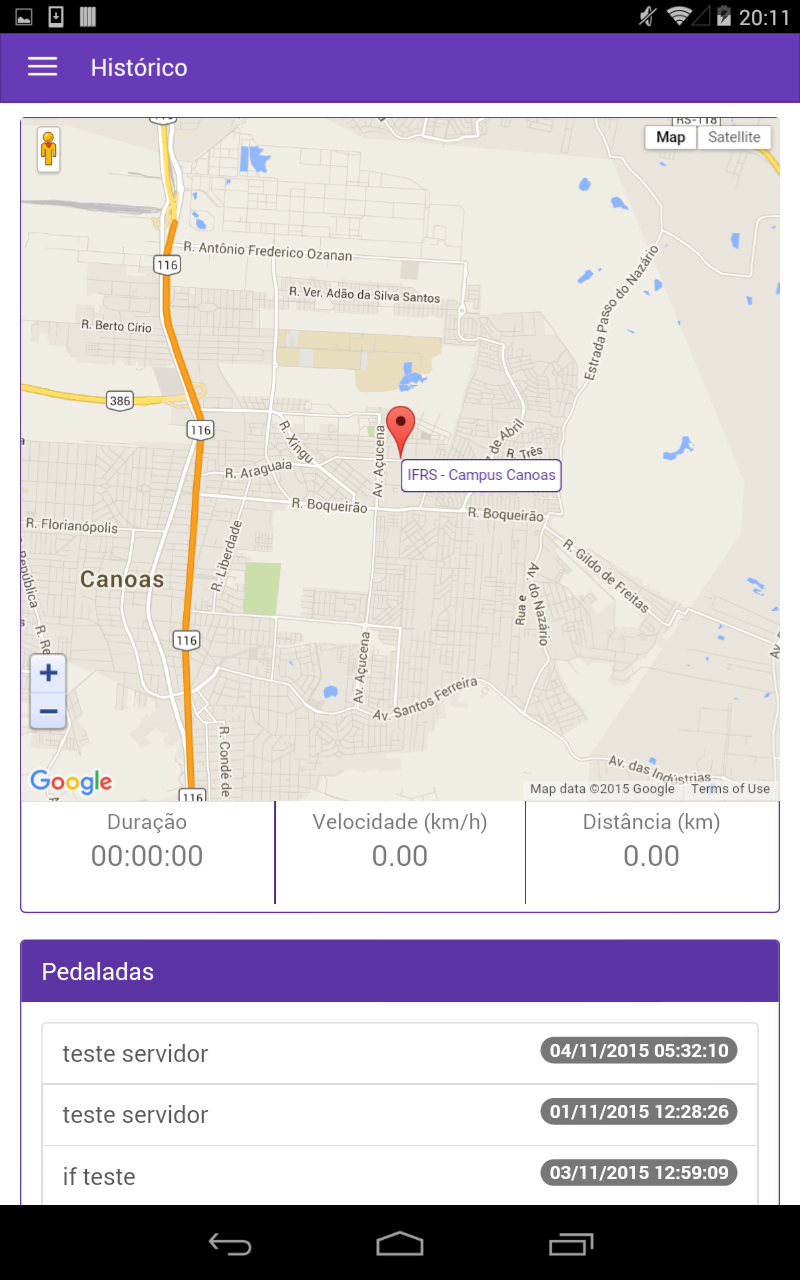
\includegraphics[width=0.95\linewidth]{figuras/p2pmaps.png}
    \label{fig:recordsMobile}
\end{minipage}%
\begin{minipage}{.7\textwidth}
    \centering
    \captionof{figure}{Histórico de pedaladas\\em telas grandes.}
    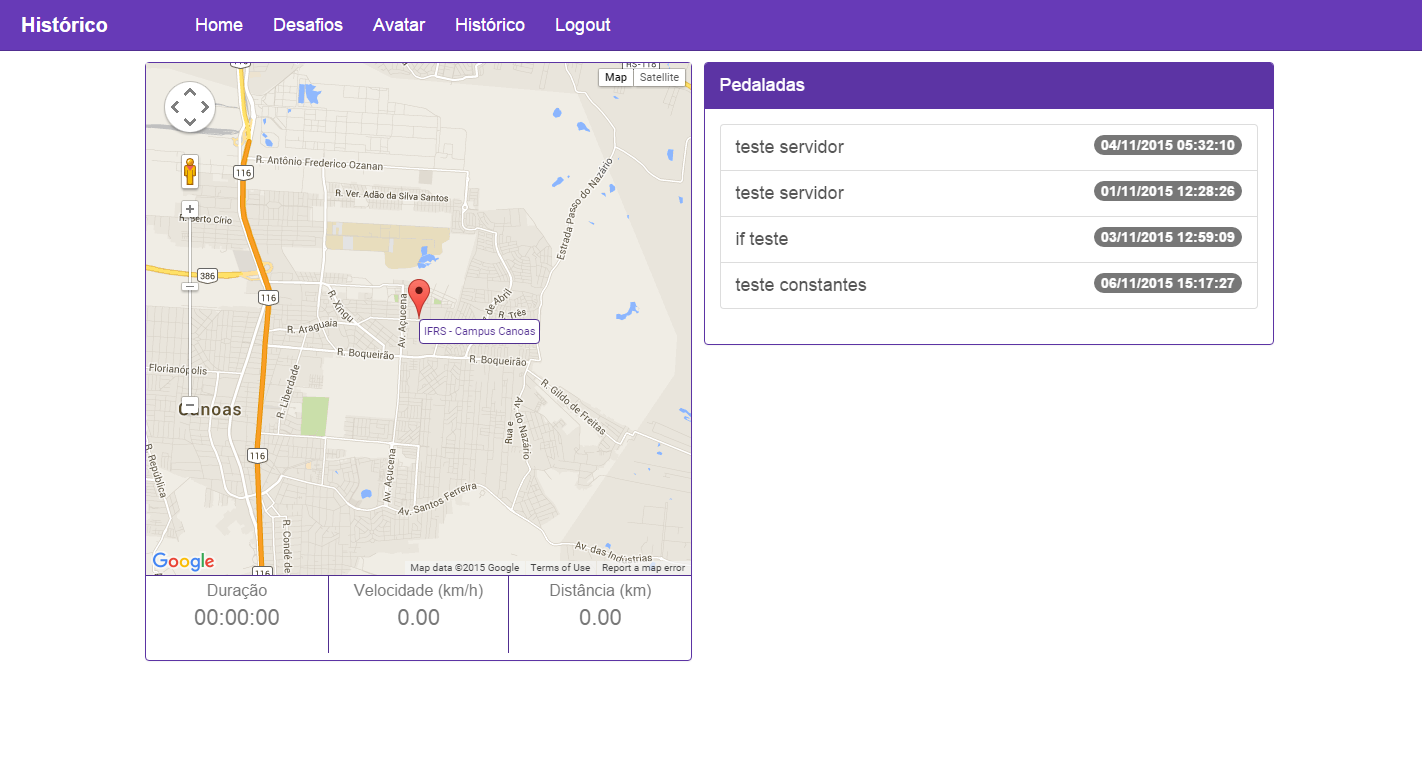
\includegraphics[width=1.1\linewidth]{figuras/p2pWebMaps.png}
    \label{fig:recordsWeb}
\end{minipage}
\par%
\bigskip
\centerline{Fonte: \textit{Print screens} do Pedal-to-Play.}
\end{figure}

Por último, a Figura \ref{fig:printMenu} apresenta o menu lateral desenvolvido usando o \textit{plugin} Jasny-Bootstrap. Este menu possibilita a navegação entre as GUI do Pedal-to-Play em telas com largura inferior a 768 \textit{pixels}. 

\begin{figure}[hb]
\begin{minipage}{.5\textwidth}
    \centering
    \captionof{figure}{GUI dos desafios.}
    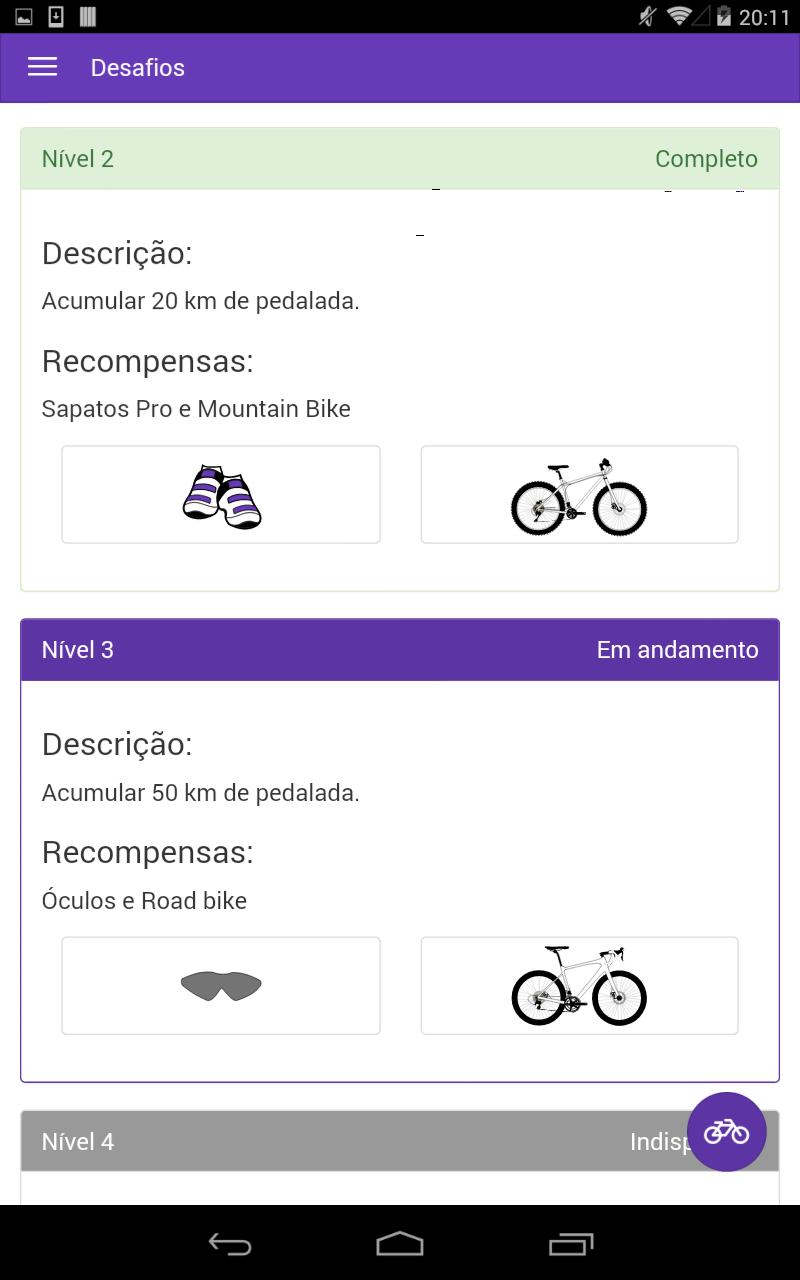
\includegraphics[width=0.5\linewidth]{figuras/p2pQuests.png}
    \label{fig:questsMobile}
\end{minipage}%
\begin{minipage}{.5\textwidth}
    \centering
    \captionof{figure}{Menu lateral para navegação.}
    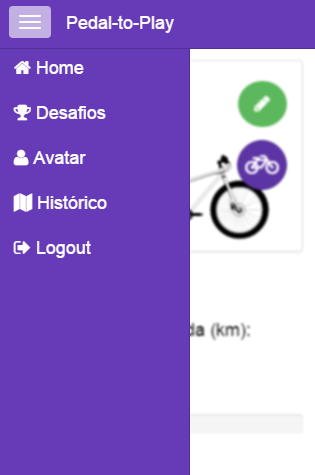
\includegraphics[width=0.5\linewidth]{figuras/p2pMenu.png}
    \label{fig:printMenu}
\end{minipage}
\par%
\bigskip
\centerline{Fonte: \textit{Print screens} do Pedal-to-Play.}
\end{figure}

\section{Teste do Monitoramento de Pedaladas}
Para verificação da funcionalidade de monitoramento de pedalada, utilizou-se os seguintes dispositivos com sistema operacional Android e com suporte à geolocalização, incluindo GPS:

\begin{enumerate}
\item Galaxy Fame Duos\footnote{\url{http://www.samsung.com/br/support/model/GT-S6812MBPZTM}}: é um modelo de \textit{smartphone} fabricado pela Samsung que conta com a versão Android 4.1.2 (Jelly Bean) e uma tela com resolução de 320 x 480 \textit{pixels}.

\item Moto G 2014\footnote{\url{http://www.motorola.com.br/Moto-G-da-Motorola/moto-g-2nd-gen-br.html}}: é um modelo de \textit{smartphone} fabricado pela Motorola que conta com a versão Android 4.4.4 (KitKat) e uma tela com resolução de 720 x 1280 \textit{pixels}.

\item Nexus 7 2012\footnote{\url{https://www.asus.com/Tablets/Nexus_7/}}: é um modelo de \textit{tablet} fabricado pela Asus que conta com a versão Android 4.4.4 (KitKat) e uma tela com resolução de 800 x 1280 \textit{pixels}.
\end{enumerate}

\subsection{Teste de Pedalada na Avenida Érico Veríssimo}
O primeiro teste ao ar livre realizado foi o monitoramento de uma pedalada rápida pela avenida Érico Veríssimo, no bairro Menino Deus, em Porto Alegre. O resultado deste teste é apresentado no mapa na Figura \ref{fig:trackErico}.

\begin{figure}[h]
\begin{minipage}{1.0\textwidth}
    \captionof{figure}{Monitoramento de pedalada na avenida Érico Veríssimo.}
    \centerline{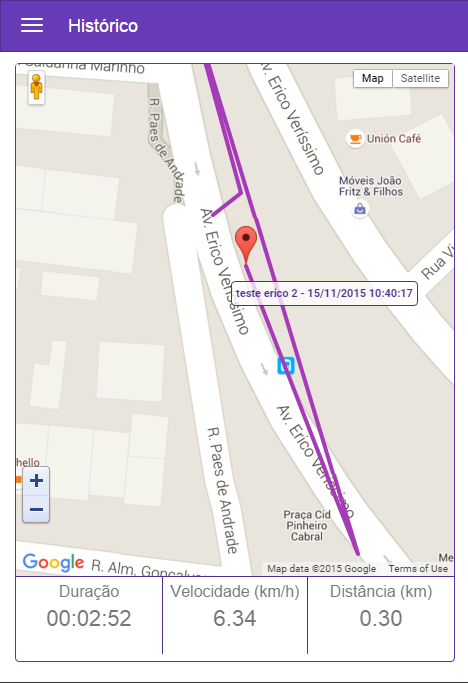
\includegraphics[width=13em]{figuras/p2pTrackErico.png}}
    \label{fig:trackErico}
\end{minipage}
\centerline{Fonte: \textit{Print screen} do Pedal-to-Play.}
\end{figure}

Como o monitoramento deste primeiro teste foi rápido, poucas posições foram capturadas pela API de geolocalização e por isso as linhas aparentam ser retas. As medidas totalizaram 300 metros de percurso, durante 2:52 minutos, resultando em uma velocidade média de 6,34 km/h. Este teste foi monitorado utilizando o Moto G.

\subsection{Teste de Pedalada no Parque Farroupilha}
O segundo teste ao ar livre foi o monitoramento de uma pedalada partindo do Parque Farroupilha até o estádio Olímpico, em Porto Alegre. O resultado deste teste é apresentado na Figura \ref{fig:trackRedencao}.

\begin{figure}[h]
\begin{minipage}{1.0\textwidth}
    \captionof{figure}{Monitoramento de pedalada no trajeto Parque Farroupilha-Olímpico.}
    \centerline{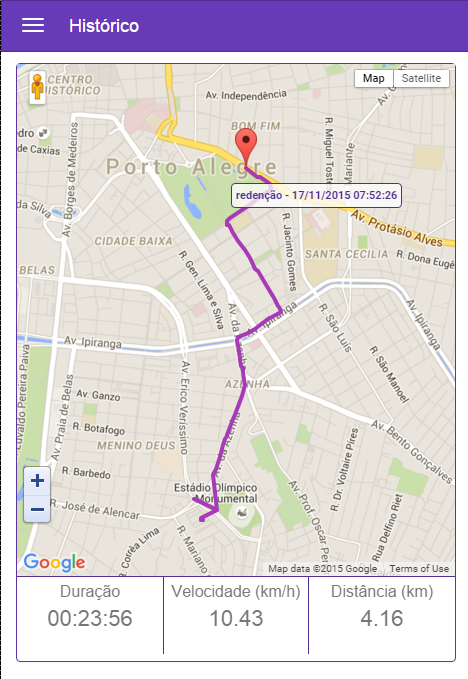
\includegraphics[width=11em]{figuras/p2pTrackRedencao.png}}
    \label{fig:trackRedencao}
\end{minipage}
\centerline{Fonte: \textit{Print screen} do Pedal-to-Play.}
\end{figure}

O teste totalizou 4,16 km de percurso, durante 23:56 minutos e uma velocidade média de 10,43 km/h. Por compreender uma pedalada mais longa do que o teste na Érico Veríssimo, o trajeto ficou mais detalhado no mapa. Para o monitoramento, utilizou-se o Galaxy Fame Duos.

\subsection{Teste sem Deslocamento}
O terceiro teste não foi ao livre e não envolveu deslocamento do usuário ou do dispositivo. O objetivo era analisar o comportamento da API de geolocalização enquanto o dispositivo está parado. Este teste foi realizado usando o Nexus 7 e seu resultado é apresentado na Figura \ref{fig:trackParado}.

\begin{figure}[h]
\begin{minipage}{1.0\textwidth}
    \captionof{figure}{\textit{Print screen} de um registro de monitoramento sem deslocamento.}
    \centerline{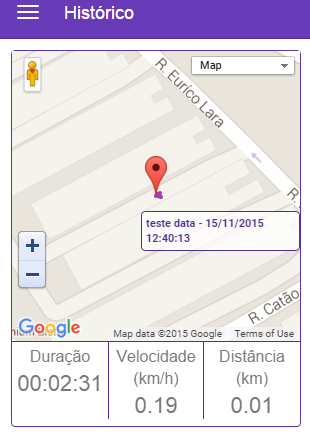
\includegraphics[width=10em]{figuras/p2pTrackParado.png}}
    \label{fig:trackParado}
\end{minipage}
\centerline{Fonte: \textit{Print screen} do Pedal-to-Play.}
\end{figure}

Como pode ser visto no \textit{print screen}, a aplicação quantificou um deslocamento de 10 metros, mesmo com o dispositivo parado. A justificativa para a API retornar posições diferentes quando não deveria é a existência de uma margem de erro, a qual é influenciada pela qualidade dos sensores no dispositivo e o nível do sinal deles. Os testes sem deslocamento foram realizados em ambientes fechados, o que compromete o sinal do GPS. Além disso, a especificação sobre Geolocalização da W3C\citeyearpar{w3cGeo} salienta que a posição retornada não tem garantia de ser verídica. Por estes fatores, trajetos curtos tendem a apresentar deformidades mais perceptíveis.
\par
O Strava detecta se o usuário está parado durante certo tempo e pausa a atividade para evitar deformidades no trajeto. Já o Runtastic não utiliza nenhum tratamento para esse fenômeno (ver teste na Figura \ref{fig:runtasticTesteParado}). 

\begin{figure}[hb]
\begin{minipage}{1.0\textwidth}
  \captionof{figure}{Registro de monitoramento sem deslocamento no Runtastic.}
  \centerline{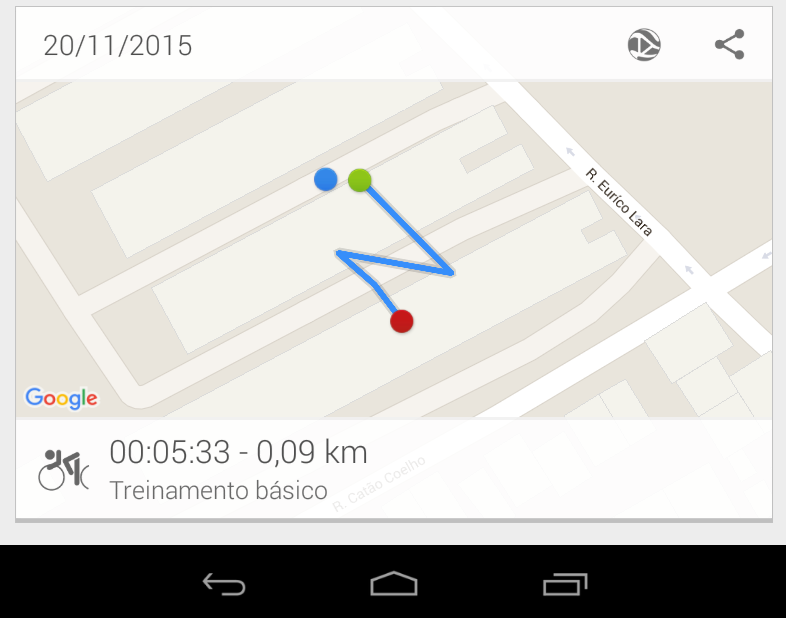
\includegraphics[width=.3\linewidth]{figuras/runtasticTesteParado.png}}
  \label{fig:runtasticTesteParado}
\end{minipage}
\par%
\bigskip
\centerline{Fonte: \textit{print screen} da aplicação Runtastic Road Bike.}
\end{figure}